\section{ PART a. Spatio-temporal Data Analysis System :}
\label{part_a}
A comprehensive system for spatio-temporal analysis requires the following components which can be broadly categorized based on their operations:
% \vspace{-4mm}

\begin{itemize}
  \item \textbf{Data Ingestion}
    {\em
    \begin{itemize}
      \item[-] Data Collection Module
    \end{itemize}
    }
  \item \textbf{Data Enrichment}
    {\em
    \begin{itemize}
    \item[-] Data Cleaning Module
    \item[-] Location Extraction Module
    \end{itemize}
    }
  \item \textbf{AI/ML Models}
    {\em
    \begin{itemize}
      \item[-] Tweet/Document Classification Module
      \item[-] Sentiment Analysis Module
      \item[-] Image Classification Module (optional)
    \end{itemize}
    }
  \item \textbf{Data Storage}
  \item \textbf{Data Processing Pipeline}
  \item \textbf{Analytics Processing Engine}
    {\em
    \begin{itemize}
      \item[-] Realtime Data Aggregation Support
      \item[-] Spatio-temporal Query Support
    \end{itemize}
    }
  \item \textbf{Visualization}
    {\em
    \begin{itemize}
      \item[-] Interactive Dashboard
    \end{itemize}
    }
\end{itemize}

In the following part I will throw some light on each component and discuss about challenges that it might have.

\subsection{Data Ingestion}
\Paragraph{Data Collection Module:}
Twitter is the biggest social media data source for researchers. Twitter's 1\% sample data stream API is the most common approach for data collection. Twitter statistics reveals that only 0.85\% of tweets in the stream is geotagged \cite{sloan2013knowing} which is significantly lower. Utmost effort and care should be taken to collect more geotagged data. Twitter's location based API should be used for such purpose.

\paragraph{Challenges:}
Collecting data from location based API or any other keyword based search API are restrictive in nature with request limit per hour.
Evading this problem might be challenging with limited resources. Multiple number of data collection servers collecting mutually exclusive geographical region can help to collect more geotagged data. For some social media sites, it is almost necessary to use proxy network to avoid IP block.

\subsection{Data Enrichment:}
\Paragraph{Data Cleaning Module:}
Data collected from social media often needs to be cleaned (e.g. tokenize, language filter etc.) for processing. The common scenarios for cleaning operations are {\em(i) filtering english tweets, (ii) removing emoticons (iii) keywords extraction etc. }

\vspace{-2mm}
\paragraph{Challenges:} There are many good tools for data cleaning. The main concerns are {\em(i) which library tools to use for desired result. (ii) the library should have high processing throughput}

\Paragraph{Location Extraction Module}
As mentioned earlier that the percentage of geotagged tweets is not high. However, a lot of attempt has been made to predict the location of the tweet based on user activity and history.  Geotagging users is now a well studied problem and it has a median error of 6.38 km which might not be very significant for our analysis\cite{compton2014geotagging}.

\vspace{-2mm}
\paragraph{Challenges:}
Increasing need to collect more data about users. If we are interested in home location of users then the above mentioned \cite{compton2014geotagging} technique is satisfactory. However, if we want the dynamic location as the users move or travel then it becomes a challenging problem.


\subsection{AI/ML Models:}
\Paragraph{Tweets/Document Classification Model:}
In order to distinguish between relevant (e.g. health, food, disease etc.) and  non relevant tweets/documents we need a tweet classification component. Unsupervised methods like topic modeling with LDA \cite{blei2003latent}, pLSA \cite{hofmann1999probabilistic} and phrase LDA \cite{el2014scalable} and modified versions of them can help in classification problem. However, microblogs classification for targeted topic needs further attention. In our work \cite{paul2017compass} for {\em Spatio-temporal Sentiment Analysis for US Election}, we used political and non-political tweet classification in a semi-supervised approach. The semi-supervised approach starts by creating training data for classification. Topic modeling act as a bootstrap method for creating training data that helps in learning tweet classification through context. This semi-supervised approach proved to be more robust \cite{paul2017compass}.

\begin{figure}[t]
	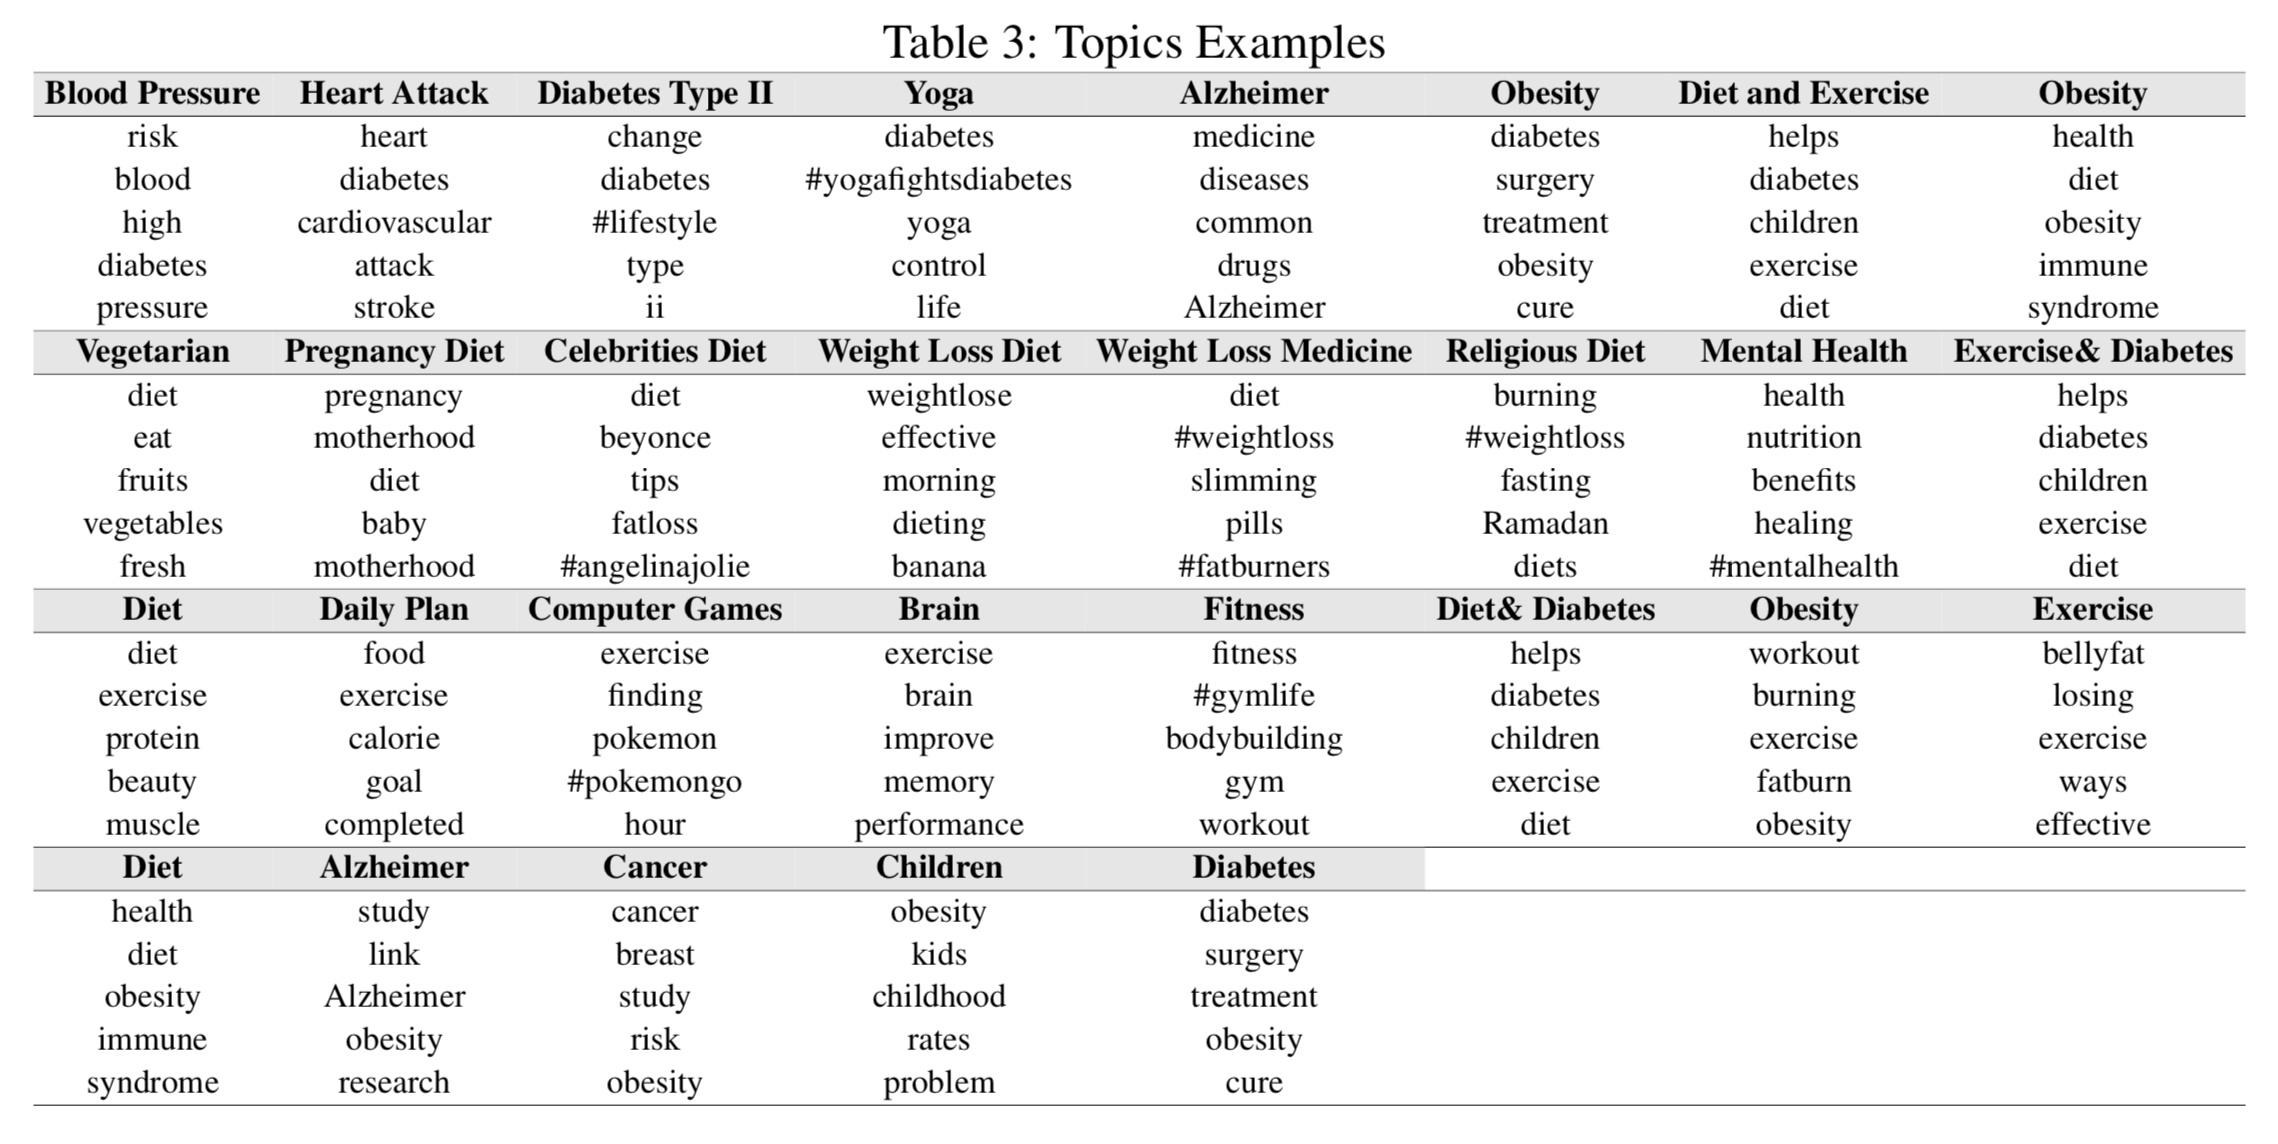
\includegraphics[width=0.99\linewidth ]{fig/HealthTopicExample.png}
    \vspace{-2mm}
    \caption{An example for topic model on ailment\cite{paul2012model}.}
    \label{fig:topic}
\end{figure}


\vspace{-2mm}
\paragraph{Challenges:}
The semi-supervised approach used in \cite{paul2017compass} have not been used yet for classification in health related topics. Previous works like {\em topic model for ailment} \cite{paul2012model} (e.g. examples of word and topic relation is shown in  Figure \ref{fig:topic}) are extension of topic modeling with LDA and specially designed for ailment tweet discovery. Remodeling semi-supervised classification for disease and health are yet to be experimented and might face challenges.
For example tweets like {``I feel like I'm going to die of Bieber Fever, No Joke!"} and  {\em ``Web design class gives me a huge headache everytime"} both tweets does not talk about health condition. Hence learning context of words is a desirable approach.

\Paragraph{Sentiment Analysis Model:}
From past decade opinion mining on text data has been a popular research topic. Pang et. al. \cite{pang2008opinion} gives a comprehensive survey on incipient opinion mining research. Twitter sentiment analysis with machine learning approaches like SVM \cite{joachims1998text}, lexicon based \cite{taboada2011lexicon}, LDA \cite{duric2012feature,kouloumpis2011twitter} and neural network \cite{dos2014deep,tang2015document} etc. Our work on {\em ``Spatio-temporal sentiment analysis on US Election"} used LSTM-RNN {\em } and FastText for achieving state-of-the-art result.

\vspace{-2mm}
\paragraph{Challenges:}
To improve upon the existing state-of-the-art methods, we have to keep adopting and experiment new AI methods. Exploration will achieve more fruitful results if proper training/ground truth datasets on sentiment are available in future. Also sentiment analysis with AI is limited to only a few language. To widespread the technology to different languages, we need resources (datasets), efforts and experiments to achieve rewarding results.


\Paragraph{Image Classification Model:}
{\em ``A picture is worth thousand words"}  is an English language-idiom that rightly characterize the scenario for tweets \cite{advice1911syracuse}. Twitter statistics reveals that 42\% of tweets attach images \cite{tweets_images}. Integrating image analysis module will reveal more information that is worth looking into.
To the best of my knowledge, we haven't yet researched a lot on public health by integrating twitter images.

\vspace{-2mm}
\paragraph{Challenges:}
Recent works on object detection from images will be our starting point \cite{girshick2014rich, mao2014deep}. We need to list the items we look out in images and provide enough example of them in training sample while training our model.


\subsection{Data Storage:}
Collected data enriched with information from ML/AI models are stored in databases. Spatio-temporal properties of data demands more attention with indexing. NoSQL key-value based databases can store all the information while the spatial indexes store object ids with location for accelerated access \cite{christensen2015storm}.

\subsection{Data Processing Pipeline:}
Creating the pipeline starting from data collection to data sink with so many
components needs expertise in data processing. In our recent work {\em AI Pro:
Data Processing Pipeline for AI models}
\footnote{\href{https://www.cs.utah.edu/~deb/aipro}{\texttt{
        https://www.cs.utah.edu/{\raise.17ex\hbox{$\scriptstyle\mathtt{\sim}$}}deb/aipro}}}
 takes care of setting up the pipeline for end users just by configuration (which is popularly known as {\em code as configuration}).
Researchers opting for customized processing pipeline will be able to create it with little or no effort.

\vspace{-2mm}
\paragraph{Challenges:}
AI Pro processing pipeline needs to adapt new technologies and support them, this requires community collaboration.

\subsection{Analytics Processing Engine:}
\Paragraph{Realtime Data Aggregation Support:}
Enriched information stored in databases is ready to be analyzed by data scientist. Data scientists finds  statistical significant information by aggregating on different attributes which is termed as slicing and dicing in data analytics world. Realtime operation of slicing and dicing with spatio-temporal operation is hard to achieve. A work from our lab by Li et. al (XDB) addresses this problem with online aggregation \cite{li2017wander}. This work is vital to achieve realtime analytics support for our system.


\vspace{-2mm}
\paragraph{Challenges:}
Scaling up the processing power in realtime environment is always a challenging task. The works mentioned above tries to solve the problem amicably. Sampling strategies on aggregate data guides data scientist to quickly
evaluate the information/statistics vital for the analysis. It is essential that sampling strategies are good enough for intended data to fetch the truthful results. That poses a challenge for the system.

\Paragraph{Spatio-temporal Query Support:}
As mentioned earlier in data storage section that geotagged data needs special attention, it is also true for query support.
Spatial operations like distance range, nearest neighbour requires special support and they are costly toward resources. Another work from our lab Xie et al. integrated {\em ``Spatial In-Memory Big data Analytics}  \cite{xie2016simba} has extended Apache Spark SQL to support spatial queries by introducing native indexing support over RDDs \cite{zaharia2012resilient}.

\subsection{Visualization:}
\Paragraph{interactive Dashboard:}
Interactive dashboard for online analysis integrated with realtime processing APIs is a feature data scientist would like to see. Filtering and selection from visualization will make the system amiable and encouraging for user. Realtime dashboard to find the rate of mentions of different topics and other time-series analysis might also be important for data scientist. STORM a spatio-temporal project from InitialDLab supports similar interface \cite{christensen2015storm}. Interactive visualization and cohesive analysis might be able to find a correlation among health, food and physical activity.

\vspace{-2mm}
\paragraph{Challenges:}
Interactive dashboard needs to be integrated with Analytics Processing API serve to fetch data with query. The tools like d3.js \footnote{\href{https://d3js.org/}{\texttt{https://d3js.org/}}} can help in designing the visualization but it requires a good skill and understanding of the subject.


\subsection{Conclusion:}
All the above mentioned components are useful and necessary for a successful analytical system on spatio-temporal system. Our system is generic in nature but can be extended with custom topic related analysis module for special purposes. For example, spatio-temporal analysis from social media might be able to throw light on public health and ailment for collective benefit of the society.


%%% Local Variables:
%%% mode: latex
%%% TeX-master: "main"
%%% End:
